\section{5 Oct 23 - Activity: Solving PDEs in Spherical
Coordinates}\label{oct-23---activity-solving-pdes-in-spherical-coordinates}

We can extend the ideas we developed from Separation of Variables to
solve PDEs in spherical coordinates. We propose a similar solution to
the one we used for Cartesian coordinates, functions of a single
variable.

\[V(r,\theta,\phi) = R(r) \Theta(\theta) \Phi(\phi)\]

We have
\href{../../assets/notes/Notes-Separation_of_Variables_Spherical.pdf}{shown
that we can solve this problem in general}. We will now apply this to a
specific problem. Recall these general solutions are written in the
following ways:

\[R(r) = A r^n + \frac{B}{r^{n+1}}\]

\[\Theta(\theta) = P^m_l(\cos\theta)\]

\[\Phi(\phi) = e^{i m \phi}\]

where \(P^m_l(\cos\theta)\) are the
\href{https://en.wikipedia.org/wiki/Associated_Legendre_polynomials}{associated
Legendre polynomials}. So that the general solution is the product of
these for different values of \(n\), \(l\), and \(m\). One solution is
some combination of \(n\), \(l\), and \(m\), written like this:

\[V_{nlm}(r,\theta,\phi) = \left(A_{nlm} r^n + \frac{B_{nlm}}{r^{n+1}}\right) P^m_l(\cos\theta) e^{i m \phi}\]

where \(A_{nlm}\) and \(B_{nlm}\) are constants. Because Laplace's
equation is linear, we can write the general solution as a sum of these
solutions:

\[V(r,\theta,\phi) = \sum_{n=0}^\infty \sum_{l=0}^\infty \sum_{m=-l}^l \left(A_{nlm} r^n + \frac{B_{nlm}}{r^{n+1}}\right) P^m_l(\cos\theta) e^{i m \phi}\]

\subsection{Visualizing the Solutions}\label{visualizing-the-solutions}

One of the major challenges with these general solutions is seeing what
the solutions look like. We can use these picture to help us dtermine if
we can remove one or more terms before trying to match boundary
conditions. We will plot each of the solutions below with respect to
their relative variables.

\subsubsection{Radial Solutions}\label{radial-solutions}

Below, we are plotting the solutions \(r^n\) and \(r^{-(n+1)}\) for
several choices of \(n\). You can see where the solutions blow up. This
is helpful for matching boundary conditions.

\begin{Shaded}
\begin{Highlighting}[]
\ImportTok{import}\NormalTok{ matplotlib.pyplot }\ImportTok{as}\NormalTok{ plt}
\ImportTok{import}\NormalTok{ numpy }\ImportTok{as}\NormalTok{ np}

\NormalTok{max\_n }\OperatorTok{=} \DecValTok{4}
\NormalTok{step }\OperatorTok{=} \DecValTok{500}
\NormalTok{max\_x }\OperatorTok{=} \DecValTok{1}
\NormalTok{start\_x }\OperatorTok{=}\NormalTok{ max\_x}\OperatorTok{/}\NormalTok{step}

\CommentTok{\# Radial coordinate}
\NormalTok{r }\OperatorTok{=}\NormalTok{ np.linspace(start\_x, max\_x, step)}

\NormalTok{plt.figure(figsize}\OperatorTok{=}\NormalTok{(}\DecValTok{10}\NormalTok{,}\DecValTok{5}\NormalTok{))}
\NormalTok{plt.subplot(}\DecValTok{1}\NormalTok{,}\DecValTok{2}\NormalTok{,}\DecValTok{1}\NormalTok{)}
\NormalTok{plt.title(}\VerbatimStringTok{r\textquotesingle{}}\DecValTok{$}\VerbatimStringTok{A\_n}\DecValTok{$}\VerbatimStringTok{ Solutions\textquotesingle{}}\NormalTok{)}
\NormalTok{plt.xlabel(}\StringTok{\textquotesingle{}r\textquotesingle{}}\NormalTok{)}
\NormalTok{plt.ylabel(}\StringTok{\textquotesingle{}R(r)\textquotesingle{}}\NormalTok{)}

\ControlFlowTok{for}\NormalTok{ n }\KeywordTok{in} \BuiltInTok{range}\NormalTok{(max\_n }\OperatorTok{+} \DecValTok{1}\NormalTok{):}
\NormalTok{    radial\_solution }\OperatorTok{=}\NormalTok{ r}\OperatorTok{**}\NormalTok{n}
\NormalTok{    plt.plot(r, radial\_solution, label}\OperatorTok{=}\SpecialStringTok{f\textquotesingle{}n=}\SpecialCharTok{\{}\NormalTok{n}\SpecialCharTok{\}}\SpecialStringTok{\textquotesingle{}}\NormalTok{)}

\NormalTok{plt.legend()}
\NormalTok{plt.grid(}\VariableTok{True}\NormalTok{)}


\NormalTok{max\_n }\OperatorTok{=} \DecValTok{4}
\NormalTok{step }\OperatorTok{=} \DecValTok{500}
\NormalTok{max\_x }\OperatorTok{=} \DecValTok{1}
\NormalTok{start\_x }\OperatorTok{=} \FloatTok{0.1}

\CommentTok{\# Radial coordinate}
\NormalTok{r }\OperatorTok{=}\NormalTok{ np.linspace(start\_x, max\_x, step)}

\NormalTok{plt.subplot(}\DecValTok{1}\NormalTok{,}\DecValTok{2}\NormalTok{,}\DecValTok{2}\NormalTok{)}
\NormalTok{plt.title(}\VerbatimStringTok{r\textquotesingle{}}\DecValTok{$}\VerbatimStringTok{B\_n}\DecValTok{$}\VerbatimStringTok{ Solutions\textquotesingle{}}\NormalTok{)}
\NormalTok{plt.xlabel(}\StringTok{\textquotesingle{}r\textquotesingle{}}\NormalTok{)}
\NormalTok{plt.ylabel(}\StringTok{\textquotesingle{}R(r)\textquotesingle{}}\NormalTok{)}

\ControlFlowTok{for}\NormalTok{ n }\KeywordTok{in} \BuiltInTok{range}\NormalTok{(max\_n }\OperatorTok{+} \DecValTok{1}\NormalTok{):  }\CommentTok{\# for negative n}

\NormalTok{    radial\_solution }\OperatorTok{=} \DecValTok{1}\OperatorTok{/}\NormalTok{(r}\OperatorTok{**}\NormalTok{(n}\OperatorTok{+}\DecValTok{1}\NormalTok{))}
\NormalTok{    plt.plot(r, radial\_solution, label}\OperatorTok{=}\SpecialStringTok{f\textquotesingle{}n=}\SpecialCharTok{\{}\NormalTok{n}\SpecialCharTok{\}}\SpecialStringTok{\textquotesingle{}}\NormalTok{)}

\NormalTok{plt.legend()}
\NormalTok{plt.grid(}\VariableTok{True}\NormalTok{)}
\end{Highlighting}
\end{Shaded}

\begin{figure}
\centering
\pandocbounded{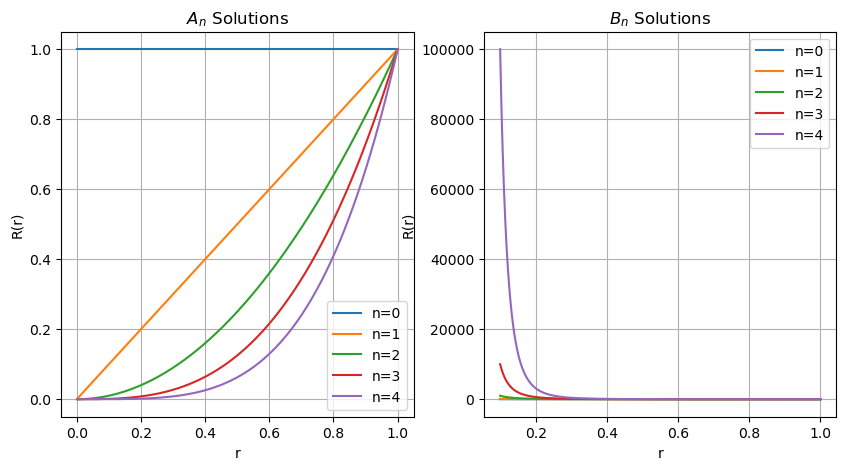
\includegraphics[keepaspectratio,alt={png}]{../images/activity-sep_var_spherical_activity-sep_var_spherical_tmp_2_0.png}}
\caption{png}
\end{figure}

\subsection{The Polar Angle Solutions}\label{the-polar-angle-solutions}

These solutions are the associated Legendre Polynomials, presented
below.

\[P_l^m(\cos\theta)\]

\begin{Shaded}
\begin{Highlighting}[]
\ImportTok{from}\NormalTok{ scipy.special }\ImportTok{import}\NormalTok{ lpmv}

\NormalTok{theta }\OperatorTok{=}\NormalTok{ np.linspace(}\DecValTok{0}\NormalTok{, np.pi, }\DecValTok{1000}\NormalTok{)  }\CommentTok{\# theta from 0 to pi}
\NormalTok{x }\OperatorTok{=}\NormalTok{ np.cos(theta)  }\CommentTok{\# x = cos(theta)}

\CommentTok{\# Define a set of (l, m) pairs to plot}
\NormalTok{lm\_pairs }\OperatorTok{=}\NormalTok{ [(}\DecValTok{0}\NormalTok{, }\DecValTok{0}\NormalTok{), (}\DecValTok{1}\NormalTok{, }\DecValTok{0}\NormalTok{), (}\DecValTok{1}\NormalTok{, }\DecValTok{1}\NormalTok{), (}\DecValTok{2}\NormalTok{, }\DecValTok{0}\NormalTok{), (}\DecValTok{2}\NormalTok{, }\DecValTok{1}\NormalTok{), (}\DecValTok{2}\NormalTok{, }\DecValTok{2}\NormalTok{), (}\DecValTok{3}\NormalTok{, }\DecValTok{0}\NormalTok{), (}\DecValTok{3}\NormalTok{, }\DecValTok{1}\NormalTok{), (}\DecValTok{3}\NormalTok{, }\DecValTok{2}\NormalTok{), (}\DecValTok{3}\NormalTok{, }\DecValTok{3}\NormalTok{)]}

\NormalTok{plt.figure(figsize}\OperatorTok{=}\NormalTok{(}\DecValTok{10}\NormalTok{,}\DecValTok{6}\NormalTok{))}
\ControlFlowTok{for}\NormalTok{ l, m }\KeywordTok{in}\NormalTok{ lm\_pairs:}
    \ControlFlowTok{if}\NormalTok{ m }\OperatorTok{\textless{}=}\NormalTok{ l:  }\CommentTok{\# The associated Legendre functions are only defined for m \textless{}= l}
\NormalTok{        plt.plot(theta, lpmv(m, l, x), label}\OperatorTok{=}\SpecialStringTok{f\textquotesingle{}$P\_}\CharTok{\{\{}\SpecialCharTok{\{}\NormalTok{l}\SpecialCharTok{\}}\CharTok{\}\}}\SpecialStringTok{\^{}}\CharTok{\{\{}\SpecialCharTok{\{}\NormalTok{m}\SpecialCharTok{\}}\CharTok{\}\}}\SpecialStringTok{$\textquotesingle{}}\NormalTok{)}

\NormalTok{plt.title(}\VerbatimStringTok{r\textquotesingle{}Polar Solutions {-} }\DecValTok{$}\VerbatimStringTok{P\_l}\DecValTok{\^{}}\VerbatimStringTok{m}\KeywordTok{(}\ErrorTok{\textbackslash{}}\VerbatimStringTok{cos}\CharTok{\textbackslash{}t}\VerbatimStringTok{heta}\KeywordTok{)}\DecValTok{$}\VerbatimStringTok{\textquotesingle{}}\NormalTok{)}
\NormalTok{plt.xlabel(}\VerbatimStringTok{r\textquotesingle{}}\DecValTok{$}\CharTok{\textbackslash{}t}\VerbatimStringTok{heta}\DecValTok{$}\VerbatimStringTok{ }\KeywordTok{(}\VerbatimStringTok{radians}\KeywordTok{)}\VerbatimStringTok{\textquotesingle{}}\NormalTok{)}
\NormalTok{plt.ylabel(}\VerbatimStringTok{r\textquotesingle{}}\DecValTok{$}\VerbatimStringTok{P\_l}\DecValTok{\^{}}\VerbatimStringTok{m}\KeywordTok{(}\ErrorTok{\textbackslash{}}\VerbatimStringTok{cos}\CharTok{\textbackslash{}t}\VerbatimStringTok{heta}\KeywordTok{)}\DecValTok{$}\VerbatimStringTok{\textquotesingle{}}\NormalTok{)}
\NormalTok{plt.legend(loc}\OperatorTok{=}\StringTok{\textquotesingle{}upper right\textquotesingle{}}\NormalTok{)}
\NormalTok{plt.grid(}\VariableTok{True}\NormalTok{)}
\end{Highlighting}
\end{Shaded}

\begin{figure}
\centering
\pandocbounded{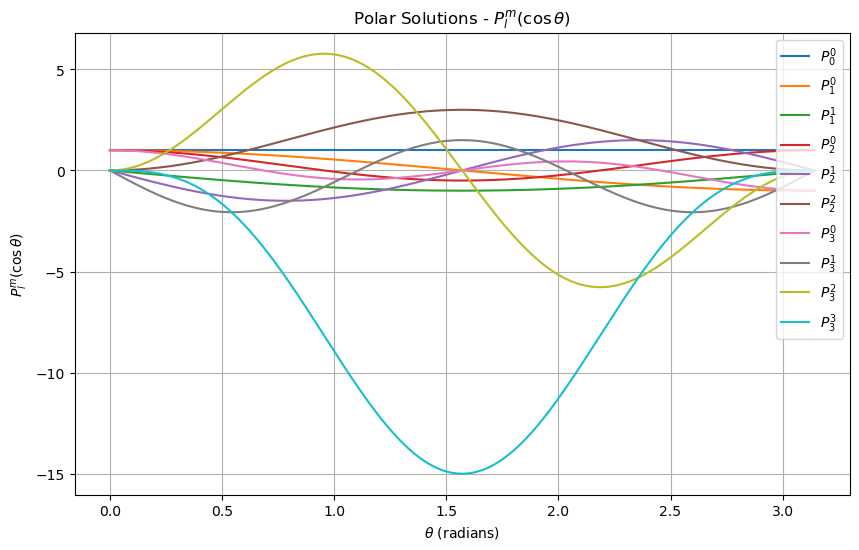
\includegraphics[keepaspectratio,alt={png}]{../images/activity-sep_var_spherical_activity-sep_var_spherical_tmp_4_0.png}}
\caption{png}
\end{figure}

\subsubsection{The Azimuthal Angle
Solutions}\label{the-azimuthal-angle-solutions}

These solutions are the exponential functions, presented below.

\[e^{i m \phi}\]

\begin{Shaded}
\begin{Highlighting}[]
\CommentTok{\# Define phi from 0 to 2*pi}
\NormalTok{phi }\OperatorTok{=}\NormalTok{ np.linspace(}\DecValTok{0}\NormalTok{, }\DecValTok{2} \OperatorTok{*}\NormalTok{ np.pi, }\DecValTok{1000}\NormalTok{)}

\CommentTok{\# Define a set of m values to plot}
\NormalTok{m\_values }\OperatorTok{=}\NormalTok{ [}\DecValTok{0}\NormalTok{, }\DecValTok{1}\NormalTok{, }\DecValTok{2}\NormalTok{]}

\NormalTok{plt.figure(figsize}\OperatorTok{=}\NormalTok{(}\DecValTok{10}\NormalTok{,}\DecValTok{6}\NormalTok{))}
\NormalTok{plt.xticks([}\DecValTok{0}\NormalTok{, np.pi}\OperatorTok{/}\DecValTok{2}\NormalTok{, np.pi, }\DecValTok{3}\OperatorTok{*}\NormalTok{np.pi}\OperatorTok{/}\DecValTok{2}\NormalTok{, }\DecValTok{2}\OperatorTok{*}\NormalTok{np.pi], [}\StringTok{\textquotesingle{}0\textquotesingle{}}\NormalTok{, }\VerbatimStringTok{r\textquotesingle{}}\DecValTok{$}\ErrorTok{\textbackslash{}}\VerbatimStringTok{pi/2}\DecValTok{$}\VerbatimStringTok{\textquotesingle{}}\NormalTok{, }\VerbatimStringTok{r\textquotesingle{}}\DecValTok{$}\ErrorTok{\textbackslash{}}\VerbatimStringTok{pi}\DecValTok{$}\VerbatimStringTok{\textquotesingle{}}\NormalTok{, }\VerbatimStringTok{r\textquotesingle{}}\DecValTok{$}\VerbatimStringTok{3}\ErrorTok{\textbackslash{}}\VerbatimStringTok{pi/2}\DecValTok{$}\VerbatimStringTok{\textquotesingle{}}\NormalTok{, }\VerbatimStringTok{r\textquotesingle{}}\DecValTok{$}\VerbatimStringTok{2}\ErrorTok{\textbackslash{}}\VerbatimStringTok{pi}\DecValTok{$}\VerbatimStringTok{\textquotesingle{}}\NormalTok{])}

\CommentTok{\# Plot the real and imaginary parts of e\^{}(im*phi) for different m values}
\ControlFlowTok{for}\NormalTok{ m }\KeywordTok{in}\NormalTok{ m\_values:}
\NormalTok{    plt.plot(phi, np.cos(m }\OperatorTok{*}\NormalTok{ phi), linestyle}\OperatorTok{=}\StringTok{\textquotesingle{}{-}\textquotesingle{}}\NormalTok{, label}\OperatorTok{=}\SpecialStringTok{f\textquotesingle{}Real, m=}\SpecialCharTok{\{}\NormalTok{m}\SpecialCharTok{\}}\SpecialStringTok{\textquotesingle{}}\NormalTok{)}

\NormalTok{plt.title(}\StringTok{\textquotesingle{}Azimuthal Solutions {-} Re($e\^{}\{im}\ErrorTok{\textbackslash{}}\StringTok{phi\}$)\textquotesingle{}}\NormalTok{)}
\NormalTok{plt.xlabel(}\VerbatimStringTok{r\textquotesingle{}}\DecValTok{$}\ErrorTok{\textbackslash{}}\VerbatimStringTok{phi}\DecValTok{$}\VerbatimStringTok{ }\KeywordTok{(}\VerbatimStringTok{radians}\KeywordTok{)}\VerbatimStringTok{\textquotesingle{}}\NormalTok{)}
\NormalTok{plt.ylabel(}\StringTok{\textquotesingle{}Value\textquotesingle{}}\NormalTok{)}
\NormalTok{plt.legend(loc}\OperatorTok{=}\StringTok{\textquotesingle{}upper right\textquotesingle{}}\NormalTok{)}
\NormalTok{plt.grid(}\VariableTok{True}\NormalTok{)}
\NormalTok{plt.show()}
\end{Highlighting}
\end{Shaded}

\begin{figure}
\centering
\pandocbounded{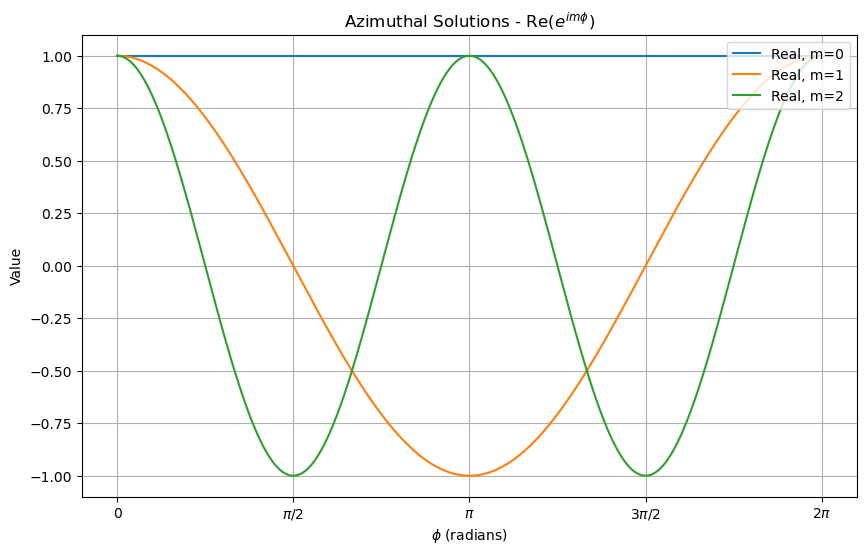
\includegraphics[keepaspectratio,alt={png}]{../images/activity-sep_var_spherical_activity-sep_var_spherical_tmp_6_0.png}}
\caption{png}
\end{figure}

\subsection{Azimuthally Symmetric
Solutions}\label{azimuthally-symmetric-solutions}

In the case of azimuthally symmetric solutions, the potential is
independent of \(\phi\) and the solutions are of the form:

\[V(r,\theta) = \sum_{n=0}^\infty \sum_{l=0}^\infty \left(A_{nl} r^n + \frac{B_{nl}}{r^{n+1}}\right) P_l(\cos\theta)\]

where \(P_l(\cos\theta)\) are the
\href{https://en.wikipedia.org/wiki/Legendre_polynomials}{Legendre
polynomials}. The solutions are plotted below, but this time in 2D. You
can imagine those solutions spun around the z-axis. We will exclusively
use these solutions for the remainder of this activity because they make
visualization easier.

We can see here why \(P_0\) is the only solution for a perfectly
spherical charge distribution. The other solutions are not spherically
symmetric. It's also possible to see where the dipole moment is in the
\(P_1\) solution; notice it's spread out a bit.

\begin{Shaded}
\begin{Highlighting}[]
\ImportTok{from}\NormalTok{ scipy.special }\ImportTok{import}\NormalTok{ legendre}

\NormalTok{theta }\OperatorTok{=}\NormalTok{ np.linspace(}\DecValTok{0}\NormalTok{, }\DecValTok{2} \OperatorTok{*}\NormalTok{ np.pi, }\DecValTok{1000}\NormalTok{)}
\NormalTok{x }\OperatorTok{=}\NormalTok{ np.cos(theta)}

\CommentTok{\# Define a set of l values to plot}
\NormalTok{l\_values }\OperatorTok{=}\NormalTok{ [}\DecValTok{0}\NormalTok{, }\DecValTok{1}\NormalTok{, }\DecValTok{2}\NormalTok{]}

\NormalTok{plt.figure(figsize}\OperatorTok{=}\NormalTok{(}\DecValTok{10}\NormalTok{,}\DecValTok{6}\NormalTok{))}

\CommentTok{\# Create a polar subplot}
\NormalTok{ax }\OperatorTok{=}\NormalTok{ plt.subplot(}\DecValTok{111}\NormalTok{, projection}\OperatorTok{=}\StringTok{\textquotesingle{}polar\textquotesingle{}}\NormalTok{)}

\ControlFlowTok{for}\NormalTok{ l }\KeywordTok{in}\NormalTok{ l\_values:}
    \CommentTok{\# Generate Legendre Polynomial}
\NormalTok{    P\_l }\OperatorTok{=}\NormalTok{ legendre(l)}
    \CommentTok{\# Evaluate the polynomial at x = cos(theta)}
\NormalTok{    y }\OperatorTok{=}\NormalTok{ P\_l(x)}
\NormalTok{    ax.plot(theta, y, label}\OperatorTok{=}\SpecialStringTok{f\textquotesingle{}$P\_}\SpecialCharTok{\{}\NormalTok{l}\SpecialCharTok{\}}\SpecialStringTok{(}\ErrorTok{\textbackslash{}}\SpecialStringTok{cos }\CharTok{\textbackslash{}\textbackslash{}}\SpecialStringTok{theta)$\textquotesingle{}}\NormalTok{)}

\NormalTok{ax.set\_title(}\StringTok{\textquotesingle{}Legendre Polynomials in Polar Coordinates\textquotesingle{}}\NormalTok{)}
\NormalTok{ax.legend(loc}\OperatorTok{=}\StringTok{\textquotesingle{}upper right\textquotesingle{}}\NormalTok{)}

\NormalTok{plt.show()}
\end{Highlighting}
\end{Shaded}

\begin{figure}
\centering
\pandocbounded{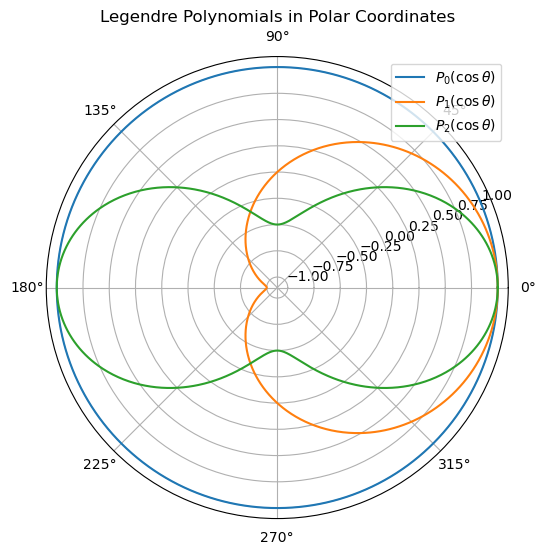
\includegraphics[keepaspectratio,alt={png}]{../images/activity-sep_var_spherical_activity-sep_var_spherical_tmp_8_0.png}}
\caption{png}
\end{figure}

\subsection{Matching Boundary Conditions and Plotting the
Potential}\label{matching-boundary-conditions-and-plotting-the-potential}

\textbf{✅ Do this}

\subsubsection{Sphere of constant surface
potential}\label{sphere-of-constant-surface-potential}

Consider a sphere of with a radius \(a\). If the potential on the
surface is \(V_0\), what is the potential inside and outside the sphere?

\begin{enumerate}
\def\labelenumi{\arabic{enumi}.}
\tightlist
\item
  Consider the radial solutions (what doesn't blow up?)
\item
  Consider the polar angle solutions, what has to be true? What does
  that say about terms with \(l>0\)?
\item
  Write down the solution inside and outside the sphere.
\item
  Make a heat map plot (in \(x\) and \(y\)) of the potential inside and
  outside the sphere. You can set \(a=1\) and \(V_0=1\) if that helps.
\end{enumerate}

\begin{Shaded}
\begin{Highlighting}[]
\CommentTok{\#\# your code here}
\end{Highlighting}
\end{Shaded}

\begin{Shaded}
\begin{Highlighting}[]

\end{Highlighting}
\end{Shaded}
